\chapter{Helyiség modellje}\label{chap:helyiseg}

% Kiindulás ssc_house_heating_system

A szabályzótervezéshez rendelkezésre kell, hogy álljon a szabályzott szakasz modellje. Ezt két részre bontottam: először az épületszerkezet, azaz a helyiség modelljét írom fel, a fűtőtestekkel a \textit{\ref{chap:futotest}. fejezetben} foglalkozom. Egy könnyen módosítható, koncentrált paraméterű hálózatot vettem fel, ahol minden elemhez lehet fizikai tartalmat rendelni. A szabályzótervezéshez a teljes modell gerjesztés-válasz kapcsolatára lesz majd szükségem.

Az energetikai jellemzők az épület energetikai tanúsítványából kiolvashatók, így a modell paraméterezhető. A tervezési lépéseket a névleges modellre elvégezve a szabályzás rögtön működőképes, nincs szükség hosszas kalibrációs időszakra beüzemelésnél. A modellbeli eltéréseket később kompenzálni lehet, mérési adatok felhasználásával.% (historikus adatok felhasználásával). %A modellben a bizonytalanságok hatása adaptív szabályozással kezelhető (lesz).

\section{A modellalkotás folyamata}
%
%White-box
%grey-box
%black-box

% zavarás, bemenet, nem irányított bemenet

A gerjesztés-válasz kapcsolatot megkaphatjuk méréssel, szimulációval vagy egyenletek felírásával. Mindegyik módszernek van előnye és hátránya is:  ha a hatásmechanizmusok pontosan ismertek, használhatunk "white-box" modellt, amiben fizikai összefüggések szerepelnek. Ha a hatásmechanizmus nem ismert, fekete dobozként ("black-box") is kezelhetjük a rendszert, de az identifikációhoz nagyon sok mérésre van szükség, hogy a mérési hibákat és zavarásokat kiküszöbölhessük.%\cite{THIEBLEMONT2017485}

Én a fizikai modell felírását választottam, melynek dinamikáját megvizsgálom a szabályozótervezéshez. Megfelelő gerjesztő jelekkel identifikálva előáll a modell átviteli függvénye (\textit{\ref{chap:ident}. fejezet}). Ehhez sokkal egyszerűbb eljutni, mint mérésekkel, mivel a Simulinkben megvalósított hálózatra az identifikáció sokkal egyszerűbb, mint valós rendszerre. A vizsgálójelek tetszőlegesen megválaszthatók, például a külső hőmérséklet hatása is pontosan meghatározható. A helyiség egy MISO (több bemenetű, egy kimenetű) rendszer, terepi méréseket használva csak hosszas mérésekből lehet szétválasztani a bemenetek (fűtés, külső hőmérséklet, napsütés) hatását a belső hőmérsékletre.

%Ha később páratartalom szabályzása is szóba kerül, még bonyolultabb a helyzet.


%\cite{SCHIRRER201686}

% --------------------------- kihúzva:
%A szakirodalomban pl. \cite{THIEBLEMONT2017485} és \cite{SCHIRRER201686} érinti ezt a kérdést:
%
%A szabályzótervezés során néhányan egyáltalán nem alkotnak modellt, csak a mért adatokat használják fel, ami eléggé időigényes: az identifikációhoz egy megfelelően nagy amplitúdójú vizsgálójelre van szükség. Viszont egy 10\si{\celsius}-kal felfűteni egy helyiséget hosszú ideig tart, ami alatt biztosan meg fog változni pl. a külső hőmérséklet. Ha a mérésekben a különböző inputok hatása a kimeneten nem különíthető el jó, az identifikáció nehéz lesz. Illetve külső hőmérséklet sem változik ugrásszerűen, a lassú időbeli változás \textit{nem jó vizsgálójel} identifikációhoz.
% ---------------------------

%Lényegében én is mért adatokat használok NEMMM, EZÉRT VAN A TANÚSÍTVÁNY!, tulajdonképpen, mivel a modellt olyan alakban kéne felírni, hogy a szabályzó azt futtatni tudja. (?)


% ---------------------------


%Vizsgálójel kiválasztása
%
%Modell struktúra kiválasztása - átviteli függvények pólusainak, zérusainak száma
%
%
%Viszont az ident toolbox tf identjénél kihasználtam azt, hogy a rendszer jellegét ismerem, azaz hogy hány pólusa és hány zérusa van a szakasznak  / felnyitott körnek. Így lett egy nagyon jól illeszkedő átviteli függvényem.
%
%Én összeraktam a fizikai modellt simulinkben (ez white-box) majd annak az ugrásválaszát mértem. Így nem egy állapotteres modell, hanem egy átviteli fv. "keletkezett".


Helyiségenkénti hőmérséklet-szabályzás esetén a belső hőmérsékletre adott egy referencia és egy mért érték.
Helyiségenként számos olyan tényező figyelembe vehető, melyek a teljes épületre különbözőek: a helyiség tájolása, az ablakok mérete, a felhasználás módja mind jobban kezelhető \textit{helyben}, mint egy központi irányítással. A helyi szabályozás referenciajeleit a lakók, dolgozók komfortérzetének megfelelően kell megadni.

A helyiség levegőjének hőmérsékletét mindenhol ugyanakkorának (homogénnek) feltételezem. A szabályzás a helyiség hőveszteségét egyenlíti ki, amit az alacsonyabb külső hőmérséklet okoz. Nem foglalkozok például szellőzésből, helyiségek közti hőmérséklet-különbségből\footnote{A modellezés egyszerűsítése végett több helyiség egymásra hatását nem veszem figyelembe.}, vagy emberek jelenlétéből származó belső zavarással.

A fűtést padlófűtés és radiátor biztosítja, mindkettőben szeleppel szabályozható az átfolyó vízmennyiség.

\section{Termikus modell}

A \textit{\ref{fig:Simscape}. ábrán} látható egy termikus mintahálózat, mellyel bemutatom a Simscape csomag elemeit, melyből a helyiség modellje is felépíthető.

A források lehetnek fix hőmérsékletű elemek (feszültségforrás) illetve hőáram forrásai (áramforrás).
%A hasonlóság nem véletlen a villamos hálózatokkal. Felfedezhető, hogy a hőáramot a hőmérséklet-különbség hozza létre, nagysága pedig fordítottan arányos a hővezetési tényezővel. 
A "vezetékek" így azonos hőmérsékletű (ekvipotenciális) pontokat kötnek össze, ezekre hőmérsékletmérőket helyezhetünk. A különböző elemekkel sorba kapcsolva helyezhetők el hőáramlást mérő blokkok.

A hőáramlást a hőellenállások korlátozzák, mivel azokon hőmérsékletesés mérhető. (Az ábrán mért hőáram a hőellenálláson eső hőmérséklettel arányos, a \textit{\ref{eq_hoaram_alap}. egyenlet} szerint.) A hőtároló elemeknek tömege és fajhője megadja a hőkapacitásukat, így ezek feltöltődhetnek, energiát tárolhatnak.


A mintahálózat egy RC-tagnak felel meg, erre a szabályzótervezés lépései a következők lennének:%\footnote{Tekintsük a mintahálózatot és az itt részletezett lépéseket egy szemléletes példának, ugyanis a szakdolgozatban tárgyalt hálózatra is ezeken a lépéseken fogok végighaladni.}:

Az identifikációnál ismert a rendszer jellege, így 0 zérussal, 1 pólussal átviteli függvényt identifikálnék.
Erre szabályzót lehetne tervezni. A szimuláció során a termikus hálózat alapjele helyére kerülne a szabályzó beavatkozó jele. A visszacsatolás a hőmérő kimenetéről történne. Ekkor, mivel a tervezés során használt modell és a  szakasz között nincs eltérés (angolul \textit{mismatch}), a szabályzás jól működik.
A paraméterek módosításával a szabályzó robusztusságát lehet tesztelni.

Ha ez a hálózat egy tényleges fizikai rendszer (például egy vízforraló) modellje lenne, akkor a szabályzás történhetne úgy, hogy a szabályzó egy beágyazott számítógépen fut, majd a teljesítményelektronikán keresztül a kívánt teljesítményt szolgáltatja, hogy például azonos hőmérsékleten tartsa benne a teát.

\begin{figure}[H]
	\begin{subfigure}[t]{\textwidth}
		\centering
		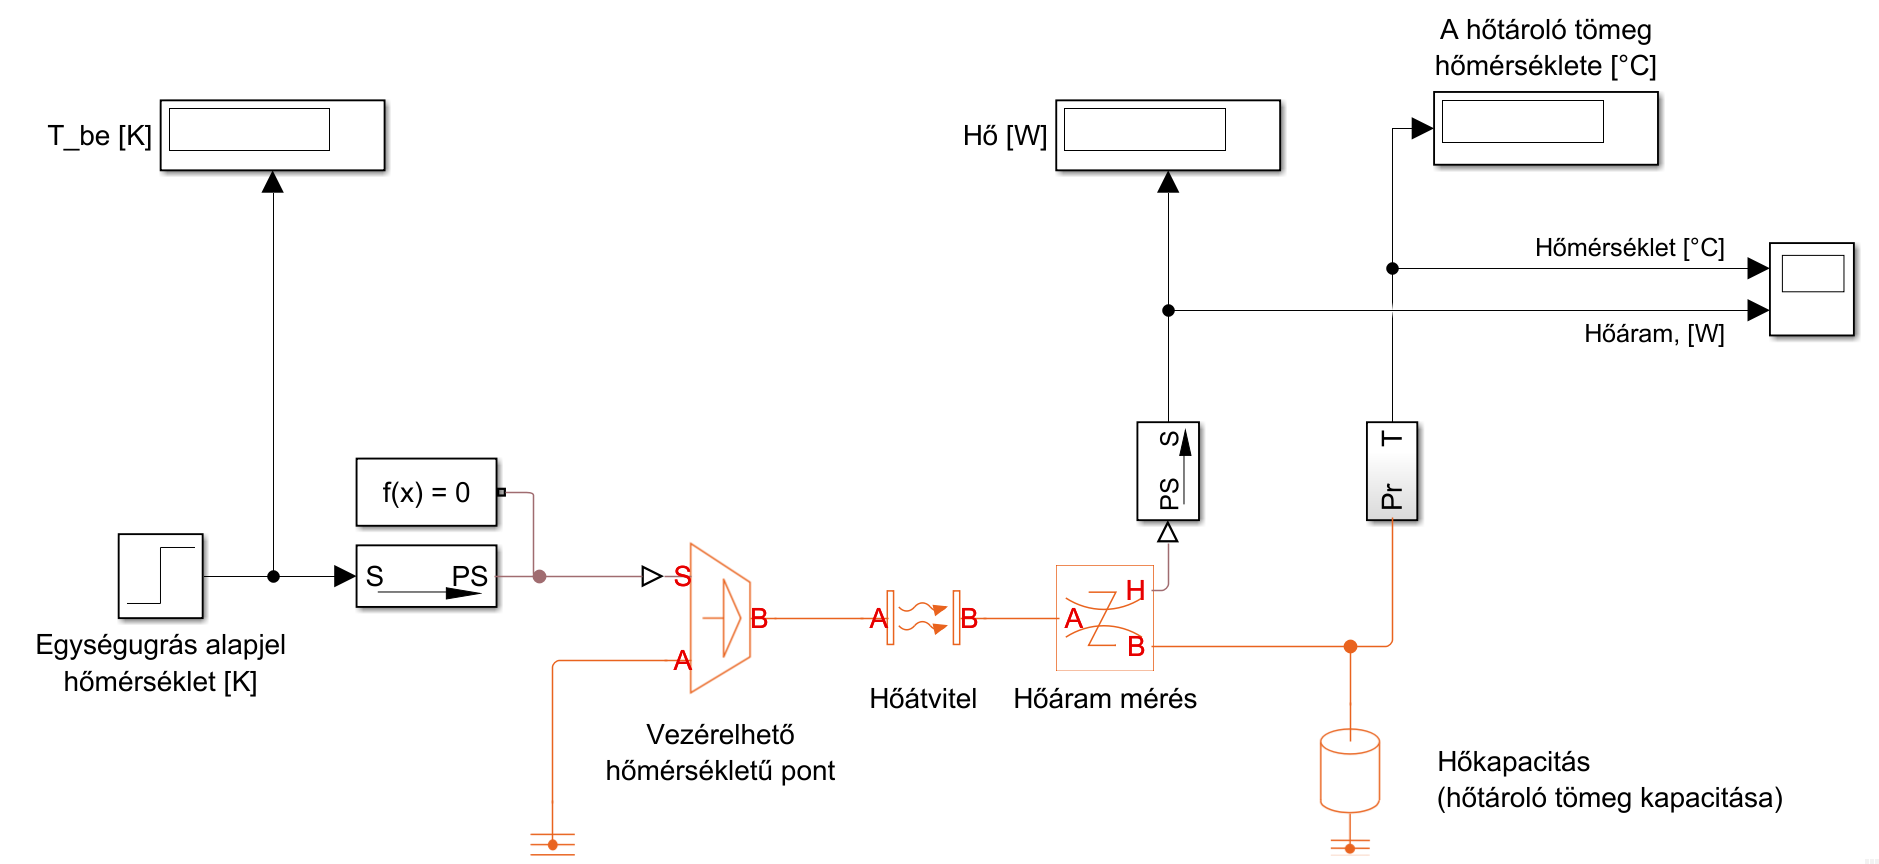
\includegraphics[width=\textwidth]{figures/SimscapeGeneral}
		\caption{Simscape termikus modell}
		\label{fig:SimscapeGeneral}
	\end{subfigure}%
	\smallskip
	\vspace*{10pt}
	\begin{subfigure}[t]{\textwidth}
		\centering
		% trim={<left> <lower> <right> <upper>}
		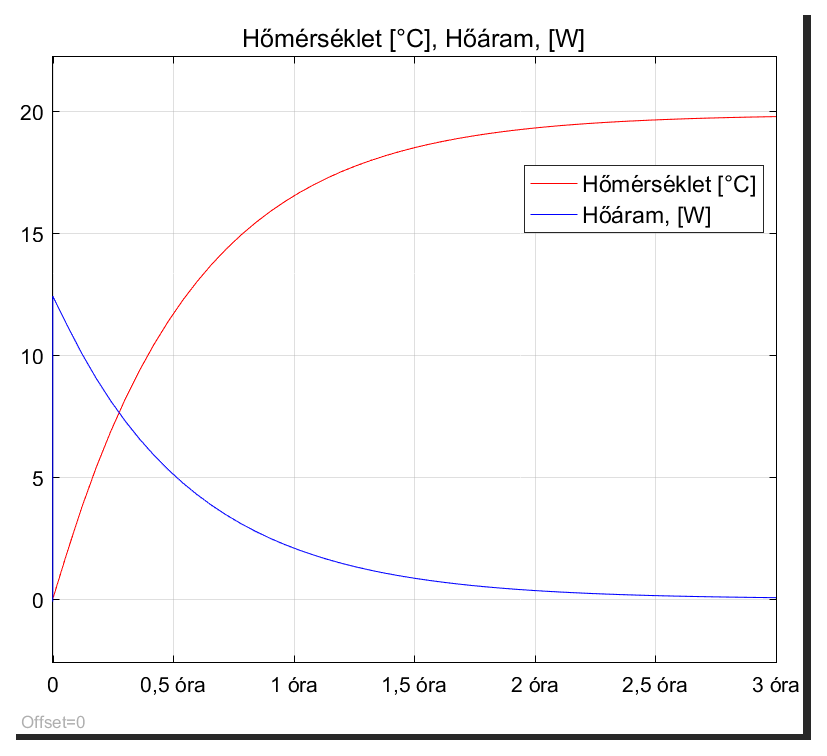
\includegraphics[trim=2 12 5 0, clip,width=0.49\textwidth]{figures/step_Simscape}
		\caption{Modell ugrásválasza}
		\label{fig:SimscapeStep}
	\end{subfigure}
	%	~
	%	\begin{subfigure}[t]{0.49\textwidth}
	%		\centering
	%%		\includegraphics[height=1.9in]{SSy}
	%%		\caption{Szimulált ugrásválasz}
	%%		\label{fig:SSy}
	%	\end{subfigure}	
	\caption{Tranziens (instacioner) hőtranszfer modellezése}
	\label{fig:Simscape}
	\centering
\end{figure}


%Természetesen lehetett volna nagyon sok állapotú állapoteres modellt is létrehozni, ám rengeteg nem mérhető belső változója lett volna, emiatt nem biztos hogy teljesen irányítható vagy megfigyelhető rendszert kaptam volna, így pedig a szabályzótervezés nem működik.


 
% \textbf{ÁBRA WHITE-BOX MODELRŐL, ÉS BLACKBOX IDENTIFIKÁCIÓRÓL. ILLETVE WHITEBOX IDENT.}



\section{Épületfizikai alapösszefüggések}
 
 A fizikai modell felírásához szükség van néhány alapösszefüggésre.
 %TODO ide még valami bevezető
 
 \subsubsection*{Hőátbocsátási tényező számítása}
 %TODO mi ez és miért jó
 A hőátadási tényező a levegő és egy felület közötti hőátadást mutatja meg,
 a rétegrendi hőátbocsátási tényező pedig számba veszi az összes réteg hatását: fal esetén annak két oldalán található levegő hőmérséklet-különbségével arányos hőáramot adja meg. 
 
 \begin{equation}\label{eq_hoatbcsatas_U}
 \begin{aligned}
 U = \frac{1}{\frac{1}{\alpha_e}+\sum\limits_{i}^{}\frac{d_i}{\lambda_i}+\frac{1}{\alpha_i}}
 \end{aligned}
 \end{equation}
 
\subsubsection*{Hővezetés, hőáramlás, hősugárzás}

A hőátadásnak három fajtája van, ezek 

\begin{equation} \label{eq_hoaram_alap}
\begin{aligned}
q = U\Delta t = \frac{\Delta t}{R}
\end{aligned}
\end{equation}

Ahol 

\begin{itemize}[itemsep=6pt,topsep=0pt,parsep=0pt,partopsep=0pt]
	\item[] $q$ a hőáram [\si[per-mode=fraction]{\watt\per\metre\squared}]
	\item[] $\Delta t$ a hőmérséklet-különbség (a potenciálkülönbség analógiájára)
	\item[] $U$ a hővezetési tényező [\si[per-mode=fraction]{\watt\per\metre\squared\per\kelvin}], reciproka az $R$ hővezetési ellenállás.
\end{itemize}


A külső falon a hőáramsűrűség:

\begin{equation}\label{eq_hoveszteseg}
\begin{aligned}
q &= U_{fal}\Delta t = \alpha_i\left(t_i-t_{i,fal}\right)
\end{aligned}
\end{equation}

Az U hőátbocsátási tényező szerepe tehát az, hogy a rétegek hatását együttesen kezelhessük. A \ref{table_house_parameters} táblázatban szerepel mindkét féle hőátadási tényező. 



\begin{table}[H]
	\footnotesize
	\centering
	\caption{Hőközlés fajtái}
	%\renewcommand{\arraystretch}{2} % to increase cell height
	%\taburulecolor{gray}
	%\begin{tabular}{|p{0.8cm}|p{1cm}|p{1cm}|p{1cm}|p{1cm}|p{1cm}|p{1cm}|p{1cm}|}
	%
	\newcolumntype{C}[1]{>{\centering\arraybackslash}p{#1}}
\newcolumntype{R}[1]{>{\raggedleft\arraybackslash}p{#1}}


\begin{tabu}{p{1.5cm}C{1.6cm}C{7cm}C{4cm}}
	%{p{1.5cm}|C{0.8cm}|C{0.8cm}|C{0.8cm}|C{0.8cm}|C{0.8cm}|C{0.8cm}|C{0.8cm}|C{0.8cm}|}
	%\multicolumn{1}{l}{}&\multicolumn{8}{l}{SDO header (első adatbyte) - master kérése}
	%\\ 		\cline{2-9}\cline{2-9}
	\hline
	\\
	& együtthatója &  a hőátadás szereplői & példa
	\\
	konvektív &  $\lambda$& áramló közeg -- szilárd anyag felülete & levegő vagy víz áramlása
	\\
	konduktív &  $h_c$&  az anyag molekulái között & az anyag belsejében
	\\
	radiatív &  $h_r$& tárgyak között, felszínükkel arányosan & hősugárzás 
	\\
%	& méret & $h_t$, átlag    & hőtároló tömeg & hőkapac
%	\\
%	& méret & $h_t$, átlag    & hőtároló tömeg & hőkapac
%	\\
%	& méret & $h_t$, átlag    & hőtároló tömeg & hőkapac
%	\\
%	& méret & $h_t$, átlag    & hőtároló tömeg & hőkapac
%	\\
%	& méret & $h_t$, átlag    & hőtároló tömeg & hőkapac
%	\\ %\hline
%	külső fal & 4.5 \si{\metre\squared} & 2 \si[per-mode=fraction]{\watt\per\metre\squared\per\kelvin} & 900kg & 756 \si[per-mode=fraction]{\kilo\joule\per\kelvin}
%	\\ %\hline
%	ablak & 4 \si{\metre\squared} & 4 \si[per-mode=fraction]{\watt\per\metre\squared\per\kelvin} & 0 & 0
%	\\ %\hline
%	belső válaszfalak & 50 \si{\metre\squared} & 7 \si[per-mode=fraction]{\watt\per\metre\squared\per\kelvin} & 5000kg & 4.2 \si[per-mode=fraction]{\mega\joule\per\kelvin}	
%	\\ %\hline
%	padló & 16 \si{\metre\squared} & 11 \si[per-mode=fraction]{\watt\per\metre\squared\per\kelvin}  & 3200kg &2.7 \si[per-mode=fraction]{\mega\joule\per\kelvin}
%	\\ %\hline
%	mennyezet & 16 \si{\metre\squared} & 5 \si[per-mode=fraction]{\watt\per\metre\squared\per\kelvin} & 3200kg &2.7 \si[per-mode=fraction]{\mega\joule\per\kelvin}	
	\\ \hline

%	belső válaszfalak & 50 \si{\metre\squared} & 7 & 50*100kg & 50*100*840		
%	\\ \hline
%	11 & Internal limit active
%	\\ \hline
%	12-13 & Operation mode specific
%	\\ \hline
%	14-15 & Reserved
\end{tabu}

	\label{tab:HeatExchangeTypes}
	%
	%\label{tab:TabularExample}
	%\tabref{TabularExample}~táblázat
\end{table}

\subsubsection*{Hőtároló képesség}

Falszerkezeteknél annak hőtároló képessége adja meg, hogy \SI{1}{\celsius}-os hőmérséklet-változás esetén mennyivel változik a szerkezet energiája. Ez az alábbi képlettel számolható:

\begin{equation}\label{eq_hotarolo}
\begin{aligned}
C &= cm\\[10pt]
E &= C\Delta T
\end{aligned}
\end{equation}

% \vspace{24pt}

% Falszerkezet, ablakszerkezet

\begin{table}[H]
	\footnotesize
	\centering
	\caption{Jelölések}
	%\renewcommand{\arraystretch}{2} % to increase cell height
	%\taburulecolor{gray}
	%\begin{tabular}{|p{0.8cm}|p{1cm}|p{1cm}|p{1cm}|p{1cm}|p{1cm}|p{1cm}|p{1cm}|}
	%
	\newcolumntype{C}[1]{>{\centering\arraybackslash}p{#1}}
\newcolumntype{R}[1]{>{\raggedleft\arraybackslash}p{#1}}

\setstretch{1.8}

\begin{tabulary}{\linewidth}{LLc}
	%\begin{tabulary}{|p{3cm}|p{1.2cm}|p{2cm}|p{3cm}|p{3cm}|}
	%{p{1.5cm}|C{0.8cm}|C{0.8cm}|C{0.8cm}|C{0.8cm}|C{0.8cm}|C{0.8cm}|C{0.8cm}|C{0.8cm}|}
	%\multicolumn{1}{l}{}&\multicolumn{8}{l}{SDO header (első adatbyte) - master kérése}
	%\\ 		\cline{2-9}\cline{2-9}
	\hline
	${Q}_{total} $& hőáram 				& \si[per-mode=fraction]{\watt} = \si[per-mode=fraction]{\joule\per\second}
	\\
	$A $		& felszín				& \si[per-mode=fraction]{\watt\per\metre\squared}
	\\
	$U$ 		& réteges szerkezet hőátbocsátási tényezője  & \si[per-mode=fraction]{\watt\per\metre\squared\per\kelvin}
	\\
	$q_{total} $& teljes hőáramsűrűség 	& \si[per-mode=fraction]{\watt\per\metre\squared}
	\\
	$h_{total}$	& teljes hőcsere együttható & \si[per-mode=fraction]{\watt\per\metre\squared\per\kelvin}
	\\
	$h_{r}$ 	& radiatív hőátadási tényező & \si[per-mode=fraction]{\watt\per\metre\squared\per\kelvin}
	\\
	$h_{c}$, $\alpha$
				& konvektív hőátadási tényező
										& \si[per-mode=fraction]{\watt\per\metre\squared\per\kelvin}
	\\
	$\lambda$  	& konduktív hőátadási tényező & \si[per-mode=fraction]{\watt\per\metre\squared\per\kelvin}
	\\
	$\varepsilon$
				& emisszivitás & --
	\\
	$t_{ref}$ 	& referencia hőmérséklet& \si[per-mode=fraction]{\celsius}
	\\
	$t_i$ 		& belső hőmérséklet 	& \si[per-mode=fraction]{\celsius}
	\\
	$t_e$ 		& külső hőmérséklet 	& \si[per-mode=fraction]{\celsius}
	\\
	$c$ 		& fajhő 		& \si[per-mode=fraction]{\joule\per\kilogram\per\kelvin}
	\\
	$C$		& hőkapacitás 		& \si[per-mode=fraction]{\joule\per\kelvin}
	\\
	$\dot{m}$ 	& tömegáram 	& \si[per-mode=fraction]{\kilogram\per\second}
	\\
	$\xi$, $u_1,u_2$
				& szelep kinyitásának mértéke [0..1]				& $\%$
	\\
	$\Delta t_m$& közepes hőmérsékletkülönbség 	& \si[per-mode=fraction]{\celsius}
	\\
	$t_i$ 		& belső hőmérséklet 	& \si[per-mode=fraction]{\celsius}

%	& méret & $h_t$, átlag    & hőtároló tömeg & hőkapac
%	\\
%	& méret & $h_t$, átlag    & hőtároló tömeg & hőkapac
%	\\
%	& méret & $h_t$, átlag    & hőtároló tömeg & hőkapac
%	\\
%	& méret & $h_t$, átlag    & hőtároló tömeg & hőkapac
%	\\
%	& méret & $h_t$, átlag    & hőtároló tömeg & hőkapac
%	\\ %\hline



%	külső fal & 4.5 \si{\metre\squared} & 2 \si[per-mode=fraction]{\watt\per\metre\squared\per\kelvin} & 900kg & 756 \si[per-mode=fraction]{\kilo\joule\per\kelvin}
%	\\ %\hline
%	ablak & 4 \si{\metre\squared} & 4 \si[per-mode=fraction]{\watt\per\metre\squared\per\kelvin} & 0 & 0
%	\\ %\hline
%	belső válaszfalak & 50 \si{\metre\squared} & 7 \si[per-mode=fraction]{\watt\per\metre\squared\per\kelvin} & 5000kg & 4.2 \si[per-mode=fraction]{\mega\joule\per\kelvin}	
%	\\ %\hline
%	padló & 16 \si{\metre\squared} & 11 \si[per-mode=fraction]{\watt\per\metre\squared\per\kelvin}  & 3200kg &2.7 \si[per-mode=fraction]{\mega\joule\per\kelvin}
%	\\ %\hline
%	mennyezet & 16 \si{\metre\squared} & 5 \si[per-mode=fraction]{\watt\per\metre\squared\per\kelvin} & 3200kg &2.7 \si[per-mode=fraction]{\mega\joule\per\kelvin}	
	\\ \hline
%	belső válaszfalak & 50 \si{\metre\squared} & 7 & 50*100kg & 50*100*840		
%	\\ \hline
%	11 & Internal limit active
%	\\ \hline
%	12-13 & Operation mode specific
%	\\ \hline
%	14-15 & Reserved
\end{tabulary}

	\label{tab:Nomenclature}
	%
	%\label{tab:TabularExample}
	%\tabref{TabularExample}~táblázat
\end{table}

\section{A megvalósított modell}

Figyelembe kell vennem a ház hőveszteségeit és hőtároló képességét is, a () és () egyenletek alapján, melynek paraméterei a \ref{table_house_parameters}. táblázatban találhatók.
%Ennek paraméterei: a határoló elemek felszíne, hőátbocsátási tényezője, a hőtároló elemek fajhője.
Az alábbi táblázat értékeinek nagy részét ki lehet tölteni a tanúsítványból. Feltételezem, hogy ez rendelkezésre áll, hiszen ennek elkészítésére elég sok esetben szükség van (adásvétel, felújítás, stb.).
Az épület éves hőigénye numerikusan is szerepel a tanúsítványban. Itt a fűtési rendszer tulajdonságain kívül a várható napsütéses órák számát és a használati melegvíz előállításának energiaigényét figyelembe veszi\footnote{A hőigény számításához törvényi előírások alapján különböző korrekciós tényezőket használnak.}.
%TODO hol van ez a törvényben?

A Matlab Simscape model és \textit{Lapusan} \cite{LAPUSAN2016320}
%\footnote{Development of a Multi-Room Building Thermodynamic Model Using Simscape Library - Ciprian Lapusan}
 hőátadásnál a réteges szerkezetekben számolt konvekcióval és kondukcióval is. Viszont ezek az adatok egyben is kezelhetők, a követelményeket ezekre a költségoptimalizált követelményszint\footnote{ A  költségoptimalizált követelményszintek megtalálhatók a 7/2006. rendelet \cite{TNM2006} 5. mellékletében.} adja meg. Régebbi épületek ezt a szintet nem tudják teljesíteni, ezekre jellemző értékeket adtam meg az alábbi táblázatban. 
%todo táblázat

Ám nem szabad összekeverni az U értéket (rétegrendi hőátbocsátási tényező) és az $\alpha_i$ konvektív hőátadási tényezőt, amit a válaszfalakra, padlóra és mennyezetre adtam meg, hiszen ezeken a modell szerint a helyiség nem veszt hőt, csak a hőtároló elemeknek adódik át.
%todo kell-e ez itt. A hőátadási tényező a levegő és egy felület közötti hőátadást mutatja meg, a rétegrendi hőátbocsátási tényező pedig számba veszi az összes réteg hatását: fal esetén annak két oldalán található levegő hőmérséklet-különbségével arányos hőáramot adja meg.

%TODO clarify - Viszont itt célszerű lenne a konvektív hőátadást is beleszámolni. 


%(Baromi érdekes, hogy nálunk otthon van egy hőcserélő a használati melegvíz és a fűtési rendszer között, annak a hatásait is lehetne nézni.)

%\begin{table}[ht]
%	\footnotesize
%	\centering
%	\caption{Az órajel-generátor chip órajel-kimenetei.} \label{tab:SysClocks}
%	\begin{tabular}{ | l | c | c |}
%		\hline
%		Órajel & Frekvencia & Cél pin \\ \hline
%		CLKA & 100 MHz & FPGA CLK0\\
%		CLKB & 48 MHz  & FPGA CLK1\\
%		CLKC & 20 MHz  & Processzor\\
%		CLKD & 25 MHz  & Ethernet chip \\
%		CLKE & 72 MHz  & FPGA CLK2\\
%		XBUF & 20 MHz  & FPGA CLK3\\
%		\hline
%	\end{tabular}
%	\label{tab:TabularExample}
%\end{table}






 A példában a Schönherz Zoltán Kollégium egy szobájának megfelelő méretű helyiséget vettem fel. Minden szobának van ablaka és külső fala, egy átlagos szobát 4 másik vesz körül. A belső falakon nem veszt hőt, csak az ablakon ill. a külső falon. Feltételezzük, hogy a radiátoros fűtést egy szeleppel szabályozhatjuk, amit tetszőleges mértékben nyithatunk ki.
 A napsütés hőnyereségét is figyelembe vehetjük.%, úgy, hogy egy hőforrás a padlót melegíti.

\section{A modell}
\begin{figure}[H]
	\centering
	% trim={<left> <lower> <right> <upper>}
	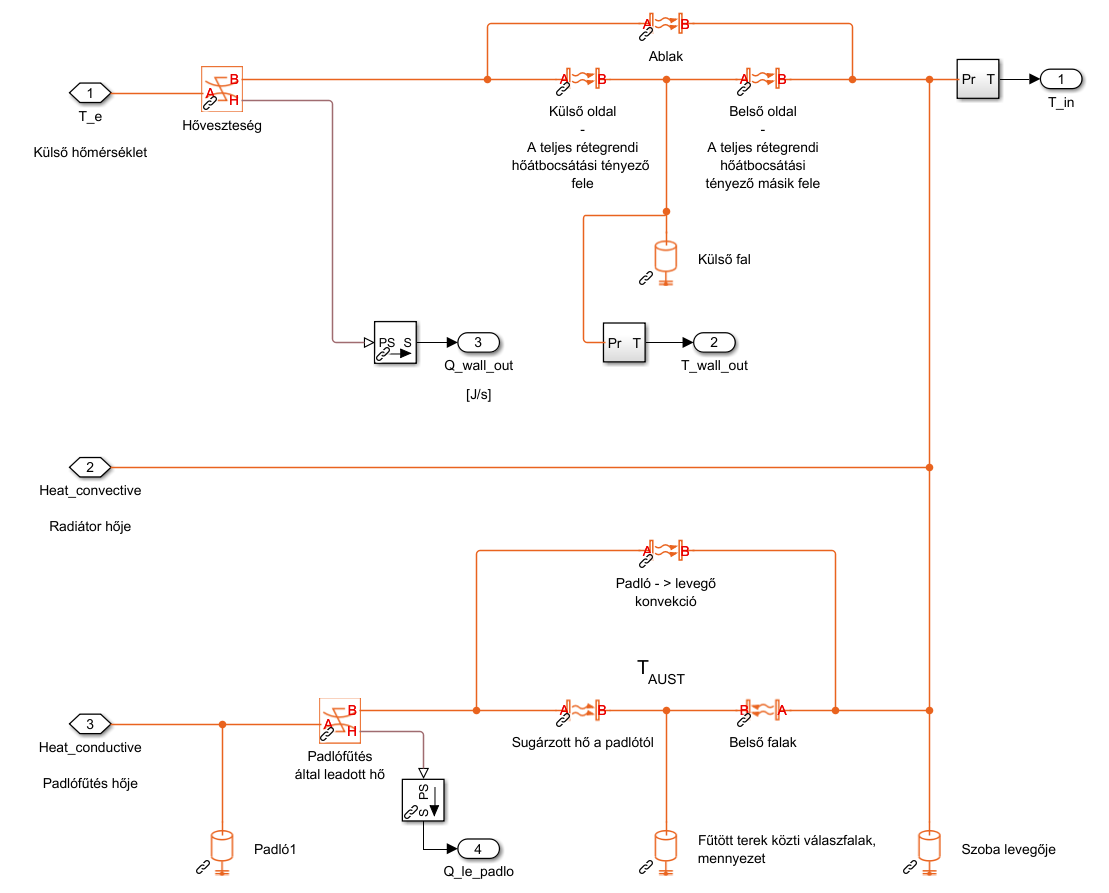
\includegraphics[trim=0 12 5 0, clip,width=\textwidth]{figures/SimscapeHouse}
	\caption{Helyiség termikus modellje}
	\label{fig:SimscapeHouse}
\end{figure}



A helyiség modellje a \textit{\ref{fig:SimscapeHouse}. ábrán} látható, három bemenete van: külső hőmérséklet, radiátor hője és a padlófűtés hője.
A külső hőmérséklet egy \say{feszültség jellegű} bemenet, hőáramot nem szab meg.
A radiátor \say{áram jellegű} kimenetet ad, hiszen itt a képlet a leadott hőt számítja: a radiátor konduktív hőárama közvetlenül a levegőt melegíti. A padlófűtés először a padlónak adja át a hőt, utána pedig a levegőnek (konduktív hőátadás), illetve a falaknak (sugárzó, radiatív hőátadás).

A levegőnek, padlónak, falaknak tömegüknél és fajhőjüknél fogva mind-mind van egy hőtároló képességük (\textit{\ref{table_house_parameters}. táblázat}), egy bizonyos idő alatt tudnak feltöltődni vagy hőenergiájukat leadni: hőmérsékletük nem változhat ugrásszerűen. %Mindezekben villamosmérnöki szemszögből felfedezhetjük az analógiát a villamos hálózatokkal.


\begin{table}[H]
	\footnotesize
	\centering
	\caption{A helyiség modelljének elemei}
	\renewcommand{\arraystretch}{2} % to increase cell height
	\taburulecolor{gray}
	
	%\begin{tabular}{|p{0.8cm}|p{1cm}|p{1cm}|p{1cm}|p{1cm}|p{1cm}|p{1cm}|p{1cm}|}
	
	\newcolumntype{C}[1]{>{\centering\arraybackslash}p{#1}}
\newcolumntype{R}[1]{>{\raggedleft\arraybackslash}p{#1}}

\begin{tabu}{@{}p{3.5cm}p{1.2cm}p{2cm}p{3cm}p{3cm}@{}}
	%\begin{tabu}{|p{3cm}|p{1.2cm}|p{2cm}|p{3cm}|p{3cm}|}
	%{p{1.5cm}|C{0.8cm}|C{0.8cm}|C{0.8cm}|C{0.8cm}|C{0.8cm}|C{0.8cm}|C{0.8cm}|C{0.8cm}|}
	%\multicolumn{1}{l}{}&\multicolumn{8}{l}{SDO header (első adatbyte) - master kérése}
	%\\ 		\cline{2-9}\cline{2-9}

	veszteséges elemek& méret & $U$    & hőtároló tömeg & hőkapacitás
	\\ \hline%\hhline{=====}
	külső fal & 4.5 \si{\metre\squared} & 2 \si[per-mode=fraction]{\watt\per\metre\squared\per\kelvin} & 900kg & 756 \si[per-mode=fraction]{\kilo\joule\per\kelvin}
	\\ %\hline
	ablak & 4 \si{\metre\squared} & 4 \si[per-mode=fraction]{\watt\per\metre\squared\per\kelvin} & - & -
	\\ %\hline
\end{tabu}
\vspace*{10pt}
\begin{tabu}{@{}p{3.5cm}p{1.2cm}p{2cm}p{3cm}p{3cm}@{}}
	csak hőtároló elemek & méret & $h_t$    & hőtároló tömeg & hőkapacitás \\	\hline%\hhline{=====}
	belső válaszfalak & 50 \si{\metre\squared} & 7 \si[per-mode=fraction]{\watt\per\metre\squared\per\kelvin} & 5000kg & 4.2 \si[per-mode=fraction]{\mega\joule\per\kelvin}	
	\\ %\hline
	padló & 16 \si{\metre\squared} & 11 \si[per-mode=fraction]{\watt\per\metre\squared\per\kelvin}  & 3200kg &2.7 \si[per-mode=fraction]{\mega\joule\per\kelvin}
	\\ %\hline
	mennyezet & 16 \si{\metre\squared} & 5 \si[per-mode=fraction]{\watt\per\metre\squared\per\kelvin} & 3200kg &2.7 \si[per-mode=fraction]{\mega\joule\per\kelvin}	
	\\ %\hline

%	belső válaszfalak & 50 \si{\metre\squared} & 7 & 50*100kg & 50*100*840		
%	\\ \hline
%	11 & Internal limit active
%	\\ \hline
%	12-13 & Operation mode specific
%	\\ \hline
%	14-15 & Reserved
\end{tabu}

	
	
	\label{table_house_parameters}
	
	%\label{tab:TabularExample}
	%\tabref{TabularExample}~táblázat
	
\end{table}


%A modell mintavételi ideje?
%A teljesítményeket megnöveljük és semmi mást, az nem lesz ekvivalens. 

\subsubsection*{Hőigény:}

A külső falon

\begin{equation}\label{eq_hoigeny}
\begin{aligned}
		Q_{ki,fal} &= U_{fal}A_{fal}\Delta T = 200\si{\watt}\\[10pt]
		Q_{ki,ablak} &= U_{ablak}A_{ablak}\Delta T = 400\si{\watt}
\end{aligned}
\end{equation}

Amennyiben a méretezési hőmérséklet $\Delta T=$ \SI{-2}{\celsius}, ami a téli átlaghőmérséklet Magyarországon.
%TODO honnan \footnote{Épületfizika kurzus alapján vettem az átlaghőmérsékletet \SI{-2}{\celsius}-nak.}


%(Gondolatkísérlet: HA nem hatna zavarás, csak az időállandók számítanának, a pontos teljesítményveszteségek, nyereségek nem. Azaz mindegy volna hogy 1000W hő szökik ki és ehhez tartozik 1500W-nyi fűtési kapacitás, vagy hogy 5000W és 7500W ezek az értékek. Ám pl. napsütés hatásakor nem csak az arányok hanem a konkrét teljesítmények is kellenek...

%Így a modell egyik belső változója bizonyosan a teljesítmény kell, hogy legyen. Erre a belső változóra hat majd zavarás: emberek jelenléte kb. \SI{80}{\watt} 1 főre, napsütés, szellőztetés, stb.)

%\hrulefill


%Erre ki kellene számítani a hőigényt, figyelembe véve azt hogy mennyi hő szökik el a külső és belső határoló felületeken keresztül.
%A gyakorlati alkalmazásokban szeretnék majd az energetikai tanúsítványból kiindulni.%, így gyakorlatilag a szoba energetikai tanúsítását végzem el - olyan szinten, amennyire nekem szükséges.


%Ashrae HVAC - 6.19 Panel H \& C. - Controls strategy
%
%A modellt a jellemző szerkezeti tulajdonságok alapján írtam fel (indoklás a táblázathoz). A modellezés Gouda alapján történik, gyakorlatilag csomóponti egyenleteket kell felírni az alábbi hálózatra, amiben az ellenállások a rétegrendi hőátbocsátási tényező reciprokai. A hőtároló képességeket kapacitások modellezik. Ezeket az elemeket Simscape-ben implementáltam, a hőáramok így áttekinthetők és a paraméterek könnyen változtathatók.
%
%A ház modelljének felírásakor figyelembe vettem a hőtároló elemeket. A pontos (reális) modell felállításakor ezek hőtartalmát (a hőáram integrálja egyensúlyi állapotban legyen 0, azaz egy nagyobb ciklusban a felvett és leadott hője egyenlő) az egyensúlyi állapothoz közelinek vettem.
%
%Viszont a szabályzótervezéshez identifikálni kell, ekkor pedig a falak, ill. szoba levegőjének kezdeti állapotát (hőmérsékletét) azonosnak vettem a külső hőmérséklettel. Így ha a hőkülönbség a modell kimenő jele, akkor lineáris a rendszer: 0 bemenetre (fűtés) 0 kimenetet ad.

%\subsection{Megvalósítás MATLAB-ban}

%a simscape elemek kapcsolatai

\section{Fűtési rendszer és ház kapcsolata}

\begin{formal}
	\textbf{Megjegyzés:}
	Ha a szabályzást egy már meglévő épületre tervezzük, akkor csak a rendszerek adatait kell felvenni, illetve identifikálni. A szakdolgozatban tárgyalt egyszerű példa során csak egy részét ismerem a paramétereknek, tehát méretezési kérdéseket is fogok érinteni.  Szerencsére az új építésű házaknál kötelező energetikai tanúsítás%\footnote{A rendelet \cite{TNM2006}
	%TODO konkrétan
	 %alapján kötelező az energetikai tanúsítvány pl. \textit{átlagos}
	 %lakóépületekre, irodákra. Adás-vételkor, felújításkor, stb.}
 egy meglehetősen részletes lajstromot ad az épület hőtechnikai tulajdonságairól. Ez alapján lehet egy hozzávetőlegesen jó modellünk az épületről, illetve a fűtési rendszerről is találhatók adatok paraméterek.

\end{formal}



 Az interneten számos tanúsító cég töltött fel minta tanúsítványokat, amiben a számítások levezetése, indoklása is megtalálható. Így az energetikai tanúsítvány lehet egy interface a szakdolgozatban bemutatott modell és a gyakorlati alkalmazások között: a valódi épület tanúsítványa alapján a modellem paraméterezhető.


Amikor a fűtési rendszer viselkedését szimulálom, nekem kell megalkotni mind a szabályzott épületrész, mind a fűtési rendszer modelljét. Így tehát ez a modellezésen felül egy méretezési feladat is, amit egy kész épületnél már elvégeztek a tervezés során, és a megfelelő fűtési teljesítmény áll rendelkezésre. %illeszkedik az igényekhez és a körülményekhez.






%
%\section{Alkalmazott fűtési rendszerek}
%
%Az alkalmazott fűtési rendszerek az épületet annak különböző pontjain gerjesztik. (Belső változóira nem egyformán hatnak: a kimeneten a változás intenzitása és sebessége más-más.) A teljes plant modell a fűtési rendszer és a ház sorba kötésével adódik.
%
%A kettő között az interface az, hogy hol avatkozunk be. Így a ház bemenetei igazából a belső változókra vonatkozó "zavarások" (a külső hőmérséklethez képest)

%\section{A modell átviteli függvénye}
%A Simulinkben identifikáltam, aztán az adatokat a sys ident toolbox-szal dolgoztam fel, tudva a modell struktúráját. (az átviteli fv. számlálójának, nevezőjének a fokszámait)

%\section{TABS}


\pagebreak
%\hrulefill